
\chapter{Discrete random variables and the binomial distribution}
\competences{define a distribution, calculate and interpret an expected value, recognise and use a binomial distribution}
\section{Reference notes}
A discrete random variable $X$ assigns a real number to each outcome. Its distribution gives the values $x_i$ and the probabilities $p_i=P(X=x_i)$, with $p_i\geq0$ and $\sum p_i=1$.

\begin{retenir}
The expected value is $E(X)=\sum_i x_ip_i$. It represents the long-run average value when the experiment is repeated under the same conditions; it is not necessarily a value actually taken by $X$.
\end{retenir}

\begin{center}
\begin{tikzpicture}[node distance=9mm and 16mm,every node/.style={draw,circle,inner sep=1.5pt,font=\small}]
\node (a) {1};
\node[below left=of a] (b) {1}; \node[below right=of a] (c) {1};
\node[below left=of b] (d) {1}; \node[below=of a] (e) {2}; \node[below right=of c] (f) {1};
\node[below left=of d] (g) {1}; \node[below left=of e] (h) {3}; \node[below right=of e] (i) {3}; \node[below right=of f] (j) {1};
\draw (a)--(b) (a)--(c) (b)--(d) (b)--(e) (c)--(e) (c)--(f) (d)--(g) (d)--(h) (e)--(h) (e)--(i) (f)--(i) (f)--(j);
\end{tikzpicture}
\end{center}

\begin{retenir}
$X$ follows a binomial distribution $\mathcal B(n,p)$ when $X$ counts the number of successes in $n$ independent Bernoulli trials with the same probability of success $p$. Then
\[
P(X=k)=\binom nk p^k(1-p)^{n-k},\qquad E(X)=np.
\]
\end{retenir}

The binomial coefficient $\binom nk$ counts the number of paths containing exactly $k$ successes among $n$ trials. For $n\leq10$, it can be read from Pascal's triangle.

\begin{center}
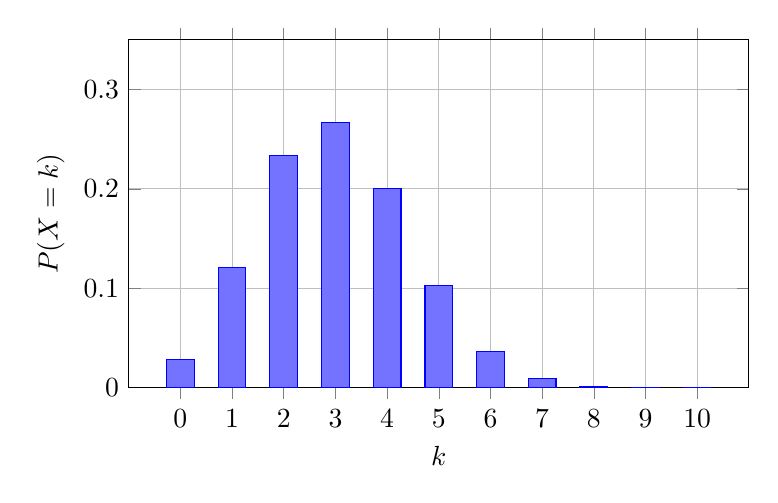
\begin{tikzpicture}
\begin{axis}[ybar,width=.78\textwidth,height=6cm,xlabel={$k$},ylabel={$P(X=k)$},ymin=0,ymax=.35,xtick=data,grid=major]
\addplot[fill=Blue!55,draw=Blue] coordinates {(0,.0282)(1,.1211)(2,.2335)(3,.2668)(4,.2001)(5,.1029)(6,.0368)(7,.0090)(8,.0015)(9,.0002)(10,.0000)};
\end{axis}
\end{tikzpicture}
\end{center}
The diagram approximately represents $\mathcal B(10,0.3)$; its centre is close to $E(X)=3$.

\sessionheader{47}{6 Apr 2027}{B: 2 h -- C: 1 h}{Expected value of a random variable}{Discrete random variables}
\begin{objectifs}\begin{itemize}\item Define a distribution.\item Calculate an expected value.\item Interpret a theoretical average.\end{itemize}\end{objectifs}
\begin{automatismes}\begin{enumerate}\item Simplify $3x+8-x+2$. \rep{$2x+10$}\item Give $E(X)$ for $X\sim\mathcal B(10,0.3)$. \rep{$3$}\item Calculate $\binom52$. \rep{$10$}\item Calculate the expected value of the constant $X$ equal to $8$. \rep{$8$}\item Express $X\geq1$ using a complement. \rep{$1-P(X=0)$}\end{enumerate}\end{automatismes}
\begin{prerequis}Reread the last written record and be able to carry out the basic calculations needed today. Before the investigation, have students rephrase the key words: define a distribution and calculate an expected value.\end{prerequis}

\begin{activite}
A game costs $2$ euros. The gross winnings are $0$, $3$ or $10$ euros with probabilities $0.6$, $0.3$, $0.1$. Construct the distribution of the net gain $X$, calculate $E(X)$ and decide whether the game is favourable to the player.

\end{activite}
\enseignant{$X$ takes the values $-2,1,8$. $E(X)=-1.2+0.3+0.8=-0.1$ euro: the game is unfavourable on average. Have students say aloud which piece of data triggers the choice of method.}

\begin{traceecrite}The distribution of $X$ assigns to each value $x_i$ the probability $p_i$. The expected value $E(X)=\sum x_ip_i$ is a theoretical long-run average.\end{traceecrite}

\begin{exemple}
Take the data from the investigation and write the solution in order: definition of the objects, property used, exact or approximate calculation, then a concluding sentence. The model answer is in the teacher edition.
\end{exemple}
\enseignant{$X$ takes the values $-2,1,8$. $E(X)=-1.2+0.3+0.8=-0.1$ euro: the game is unfavourable on average.}

\begin{exercice}[-- essential]
\begin{enumerate}\item Justify that the number of successes among $8$ independent trials, with $p=0.3$, follows a binomial distribution.\item Calculate $P(X=2)$ and $P(X=0)$.\item Deduce $P(X\geq1)$ and calculate $E(X)$.\end{enumerate}
\end{exercice}
\enseignant{$X\sim\mathcal B(8,0.3)$. $P(X=2)=\binom{8}2 0.3^2 0.7^{6}$, $P(X=0)=0.7^{8}$, $P(X\geq1)=1-P(X=0)$ and $E(X)=\dfrac{24}{10}$.}

\manuelref{Calao, course pp. 154--159; exercises p. 160, no.~1--5}
\CalaoSession{47}

\begin{dm}Redo practice exercise 2 with the following data: replace the initial value by $355$ and the rate or common ratio by $7$. Write it up in four lines: data, formula, calculation, conclusion.\end{dm}
\enseignant{The solution depends on the exercise redone. Check above all the consistency of the model, the number of iterations, the rounding and the concluding sentence.}

\begin{sortie}On a half-sheet: write the main rule of the session, work through a very short example and give a confidence level from 1 to 4. Essential question(s) of the day: 1, 2 and 3.\end{sortie}

\ifprof
\begin{methode}
\textbf{1 h session:} 7 min of fluency; 10 min of pooling and written record; 28 min of essential exercises; 5 min of correction; 3 min of exit ticket.\\
\textbf{2 h session:} add 20 min of investigation, 20 min of formalisation, a second independent exercise and 10 min of comparative correction.\\
\textbf{Differentiation:} give struggling students a four-box sheet (data, model, calculation, conclusion). Ask quick students to produce a counterexample, a justification or a second method.
\end{methode}
\fi
\sessionheader{48}{8 Apr 2027}{B: 1 h -- C: 2 h}{Binomial distribution: recognising a situation}{Discrete random variables}
\begin{objectifs}\begin{itemize}\item Recognise a Bernoulli scheme.\item Identify $n$ and $p$.\item Define $X$.\end{itemize}\end{objectifs}
\begin{automatismes}\begin{enumerate}\item Calculate $5\,\%$ of $180$. \rep{$9$}\item Calculate $\binom52$. \rep{$10$}\item Calculate the expected value of the constant $X$ equal to $9$. \rep{$9$}\item Express $X\geq1$ using a complement. \rep{$1-P(X=0)$}\item Give $E(X)$ for $X\sim\mathcal B(10,0.3)$. \rep{$3$}\end{enumerate}\end{automatismes}
\begin{prerequis}Reread the last written record and be able to carry out the basic calculations needed today. Before the investigation, have students rephrase the key words: recognise a Bernoulli scheme and identify $n$ and $p$.\end{prerequis}

\begin{activite}
A customer accepts an offer with probability $0.25$. An adviser contacts eight customers independently. Define $X$, justify the binomial distribution and identify $n$ and $p$.

\end{activite}
\enseignant{$X$ counts the acceptances; repetition of 8 identical and independent trials, success with probability $0.25$: $X\sim\mathcal B(8,0.25)$. Have students say aloud which piece of data triggers the choice of method.}

\begin{traceecrite}$X\sim\mathcal B(n,p)$ if $X$ counts the successes in $n$ independent trials with the same probability $p$.\end{traceecrite}

\begin{exemple}
Take the data from the investigation and write the solution in order: definition of the objects, property used, exact or approximate calculation, then a concluding sentence. The model answer is in the teacher edition.
\end{exemple}
\enseignant{$X$ counts the acceptances; repetition of 8 identical and independent trials, success with probability $0.25$: $X\sim\mathcal B(8,0.25)$.}

\begin{exercice}[-- essential]
\begin{enumerate}\item Justify that the number of successes among $9$ independent trials, with $p=0.3$, follows a binomial distribution.\item Calculate $P(X=2)$ and $P(X=0)$.\item Deduce $P(X\geq1)$ and calculate $E(X)$.\end{enumerate}
\end{exercice}
\enseignant{$X\sim\mathcal B(9,0.3)$. $P(X=2)=\binom{9}2 0.3^2 0.7^{7}$, $P(X=0)=0.7^{9}$, $P(X\geq1)=1-P(X=0)$ and $E(X)=\dfrac{27}{10}$.}

\manuelref{Calao, course pp. 154--159; exercises p. 160, no.~5, then p. 162, no.~14--20}
\CalaoSession{48}

\begin{dm}Redo practice exercise 3 with the following data: replace the initial value by $360$ and the rate or common ratio by $2$. Write it up in four lines: data, formula, calculation, conclusion.\end{dm}
\enseignant{The solution depends on the exercise redone. Check above all the consistency of the model, the number of iterations, the rounding and the concluding sentence.}

\begin{sortie}On a half-sheet: write the main rule of the session, work through a very short example and give a confidence level from 1 to 4. Essential question(s) of the day: 1 and 2.\end{sortie}

\ifprof
\begin{methode}
\textbf{1 h session:} 7 min of fluency; 10 min of pooling and written record; 28 min of essential exercises; 5 min of correction; 3 min of exit ticket.\\
\textbf{2 h session:} add 20 min of investigation, 20 min of formalisation, a second independent exercise and 10 min of comparative correction.\\
\textbf{Differentiation:} give struggling students a four-box sheet (data, model, calculation, conclusion). Ask quick students to produce a counterexample, a justification or a second method.
\end{methode}
\fi
\sessionheader{49}{27 Apr 2027}{B: 2 h -- C: 1 h}{Pascal's triangle and binomial coefficients}{Discrete random variables}
\begin{objectifs}\begin{itemize}\item Build Pascal's triangle.\item Read $\binom nk$.\item Interpret a coefficient.\end{itemize}\end{objectifs}
\begin{automatismes}\begin{enumerate}\item Write the multiplier for an increase of $10\,\%$. \rep{$1+\dfrac{10}{100}=1.10$}\item Calculate the expected value of the constant $X$ equal to $3$. \rep{$3$}\item Express $X\geq1$ using a complement. \rep{$1-P(X=0)$}\item Give $E(X)$ for $X\sim\mathcal B(10,0.3)$. \rep{$3$}\item Calculate $\binom52$. \rep{$10$}\end{enumerate}\end{automatismes}
\begin{prerequis}Reread the last written record and be able to carry out the basic calculations needed today. Before the investigation, have students rephrase the key words: build Pascal's triangle and read $\binom nk$.\end{prerequis}

\begin{activite}
Build rows $n=0$ to $n=6$ of Pascal's triangle. Explain the calculation of the number $15$ in row $6$, then read $\binom62$ and $\binom64$.
\begin{center}\begin{tabular}{*{9}{c}}&&&&1&&&&\\&&&1&&1&&&\\&&1&&2&&1&&\\&1&&3&&3&&1&\\1&&4&&6&&4&&1\end{tabular}\end{center}
\end{activite}
\enseignant{Each interior number is the sum of the two numbers above it. $\binom62=\binom64=15$. Have students say aloud which piece of data triggers the choice of method.}

\begin{traceecrite}Pascal's triangle satisfies $\binom nk=\binom{n-1}{k-1}+\binom{n-1}{k}$. The edges equal $1$.\end{traceecrite}

\begin{exemple}
Take the data from the investigation and write the solution in order: definition of the objects, property used, exact or approximate calculation, then a concluding sentence. The model answer is in the teacher edition.
\end{exemple}
\enseignant{Each interior number is the sum of the two numbers above it. $\binom62=\binom64=15$.}

\begin{exercice}[-- essential]
\begin{enumerate}\item Justify that the number of successes among $10$ independent trials, with $p=0.3$, follows a binomial distribution.\item Calculate $P(X=2)$ and $P(X=0)$.\item Deduce $P(X\geq1)$ and calculate $E(X)$.\end{enumerate}
\end{exercice}
\enseignant{$X\sim\mathcal B(10,0.3)$. $P(X=2)=\binom{10}2 0.3^2 0.7^{8}$, $P(X=0)=0.7^{10}$, $P(X\geq1)=1-P(X=0)$ and $E(X)=\dfrac{30}{10}$.}

\manuelref{Calao, p. 164, no.~24--29, then p. 166, no.~36}
\CalaoSession{49}

\begin{dm}Redo practice exercise 2 with the following data: replace the initial value by $365$ and the rate or common ratio by $3$. Write it up in four lines: data, formula, calculation, conclusion.\end{dm}
\enseignant{The solution depends on the exercise redone. Check above all the consistency of the model, the number of iterations, the rounding and the concluding sentence.}

\begin{sortie}On a half-sheet: write the main rule of the session, work through a very short example and give a confidence level from 1 to 4. Essential question(s) of the day: 1, 2 and 3.\end{sortie}

\ifprof
\begin{methode}
\textbf{1 h session:} 7 min of fluency; 10 min of pooling and written record; 28 min of essential exercises; 5 min of correction; 3 min of exit ticket.\\
\textbf{2 h session:} add 20 min of investigation, 20 min of formalisation, a second independent exercise and 10 min of comparative correction.\\
\textbf{Differentiation:} give struggling students a four-box sheet (data, model, calculation, conclusion). Ask quick students to produce a counterexample, a justification or a second method.
\end{methode}
\fi
\sessionheader{50}{29 Apr 2027}{B: 1 h -- C: 2 h}{Binomial probabilities}{Discrete random variables}
\begin{objectifs}\begin{itemize}\item Calculate $P(X=k)$.\item Translate at least/at most.\item Use the complement.\end{itemize}\end{objectifs}
\begin{automatismes}\begin{enumerate}\item Simplify $3x+4-x+2$. \rep{$2x+6$}\item Express $X\geq1$ using a complement. \rep{$1-P(X=0)$}\item Give $E(X)$ for $X\sim\mathcal B(10,0.3)$. \rep{$3$}\item Calculate $\binom52$. \rep{$10$}\item Calculate the expected value of the constant $X$ equal to $4$. \rep{$4$}\end{enumerate}\end{automatismes}
\begin{prerequis}Reread the last written record and be able to carry out the basic calculations needed today. Before the investigation, have students rephrase the key words: calculate $p(x=k)$ and translate at least/at most.\end{prerequis}

\begin{activite}
For $X\sim\mathcal B(8,0.25)$, calculate $P(X=2)$, $P(X=0)$, then $P(X\geq1)$. Translate each event into a sentence.
\begin{center}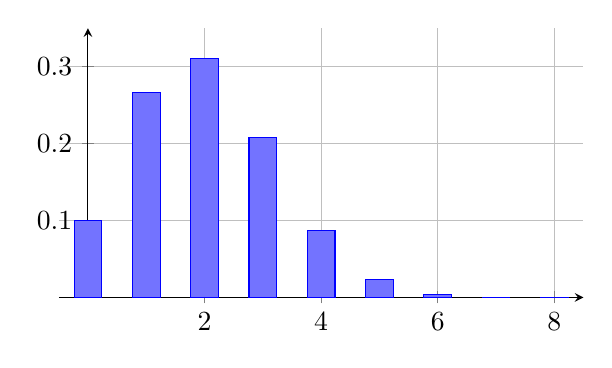
\begin{tikzpicture}\begin{axis}[width=.68\textwidth,height=5cm,axis lines=middle,xmin=-.5,xmax=8.5,ymin=0,ymax=.35,grid=major]\addplot[ybar,fill=Blue!55,draw=Blue] coordinates {(0,.10)(1,.267)(2,.311)(3,.208)(4,.087)(5,.023)(6,.004)(7,.0004)(8,.00002)};\end{axis}\end{tikzpicture}\end{center}
\end{activite}
\enseignant{$P(X=2)=\binom82 0.25^2 0.75^6\approx0.3115$; $P(X=0)=0.75^8\approx0.1001$; $P(X\geq1)\approx0.8999$. Have students say aloud which piece of data triggers the choice of method.}

\begin{traceecrite}If $X\sim\mathcal B(n,p)$, then $P(X=k)=\binom nkp^k(1-p)^{n-k}$. Translate ``at least'', ``at most'' and ``none'' carefully.\end{traceecrite}

\begin{exemple}
Take the data from the investigation and write the solution in order: definition of the objects, property used, exact or approximate calculation, then a concluding sentence. The model answer is in the teacher edition.
\end{exemple}
\enseignant{$P(X=2)=\binom82 0.25^2 0.75^6\approx0.3115$; $P(X=0)=0.75^8\approx0.1001$; $P(X\geq1)\approx0.8999$.}

\begin{exercice}[-- essential]
\begin{enumerate}\item Justify that the number of successes among $6$ independent trials, with $p=0.3$, follows a binomial distribution.\item Calculate $P(X=2)$ and $P(X=0)$.\item Deduce $P(X\geq1)$ and calculate $E(X)$.\end{enumerate}
\end{exercice}
\enseignant{$X\sim\mathcal B(6,0.3)$. $P(X=2)=\binom{6}2 0.3^2 0.7^{4}$, $P(X=0)=0.7^{6}$, $P(X\geq1)=1-P(X=0)$ and $E(X)=\dfrac{18}{10}$.}

\manuelref{Calao, p. 164, no.~24--29, then p. 168, no.~41--45}
\CalaoSession{50}

\begin{dm}Redo practice exercise 3 with the following data: replace the initial value by $370$ and the rate or common ratio by $4$. Write it up in four lines: data, formula, calculation, conclusion.\end{dm}
\enseignant{The solution depends on the exercise redone. Check above all the consistency of the model, the number of iterations, the rounding and the concluding sentence.}

\begin{sortie}On a half-sheet: write the main rule of the session, work through a very short example and give a confidence level from 1 to 4. Essential question(s) of the day: 1 and 2.\end{sortie}

\ifprof
\begin{methode}
\textbf{1 h session:} 7 min of fluency; 10 min of pooling and written record; 28 min of essential exercises; 5 min of correction; 3 min of exit ticket.\\
\textbf{2 h session:} add 20 min of investigation, 20 min of formalisation, a second independent exercise and 10 min of comparative correction.\\
\textbf{Differentiation:} give struggling students a four-box sheet (data, model, calculation, conclusion). Ask quick students to produce a counterexample, a justification or a second method.
\end{methode}
\fi
\sessionheader{51}{4 May 2027}{B: 2 h -- C: 1 h}{Chapter review and test}{Discrete random variables}
\begin{objectifs}\begin{itemize}\item Calculate and interpret $E(X)$.\item Solve a binomial problem.\item Analyse one's mistakes.\end{itemize}\end{objectifs}
\begin{automatismes}\begin{enumerate}\item Calculate $20\,\%$ of $100$. \rep{$20$}\item Give $E(X)$ for $X\sim\mathcal B(10,0.3)$. \rep{$3$}\item Calculate $\binom52$. \rep{$10$}\item Calculate the expected value of the constant $X$ equal to $5$. \rep{$5$}\item Express $X\geq1$ using a complement. \rep{$1-P(X=0)$}\end{enumerate}\end{automatismes}
\begin{prerequis}Reread the last written record and be able to carry out the basic calculations needed today. Before the investigation, have students rephrase the key words: calculate and interpret $e(x)$ and solve a binomial problem.\end{prerequis}

\begin{activite}
A centre receives $120$ groups of $10$ customers, each customer complaining with probability $0.08$. Estimate the average number of complaints per group, then over all the groups. Discuss what the expected value does and does not allow us to predict.

\end{activite}
\enseignant{Per group $E(X)=10\times0.08=0.8$. Over 120 groups, about $96$ complaints on average; this is not a certainty. Have students say aloud which piece of data triggers the choice of method.}

\begin{traceecrite}For $X\sim\mathcal B(n,p)$, $E(X)=np$. The value gives the average number of successes over a large number of series of $n$ trials.\end{traceecrite}

\begin{exemple}
Take the data from the investigation and write the solution in order: definition of the objects, property used, exact or approximate calculation, then a concluding sentence. The model answer is in the teacher edition.
\end{exemple}
\enseignant{Per group $E(X)=10\times0.08=0.8$. Over 120 groups, about $96$ complaints on average; this is not a certainty.}

\begin{exercice}[-- essential]
\begin{enumerate}\item Justify that the number of successes among $7$ independent trials, with $p=0.3$, follows a binomial distribution.\item Calculate $P(X=2)$ and $P(X=0)$.\item Deduce $P(X\geq1)$ and calculate $E(X)$.\end{enumerate}
\end{exercice}
\enseignant{$X\sim\mathcal B(7,0.3)$. $P(X=2)=\binom{7}2 0.3^2 0.7^{5}$, $P(X=0)=0.7^{7}$, $P(X\geq1)=1-P(X=0)$ and $E(X)=\dfrac{21}{10}$.}

\manuelref{Calao, pp. 160--169}
\CalaoSession{51}

\begin{dm}Redo practice exercise 2 with the following data: replace the initial value by $375$ and the rate or common ratio by $5$. Write it up in four lines: data, formula, calculation, conclusion.\end{dm}
\enseignant{The solution depends on the exercise redone. Check above all the consistency of the model, the number of iterations, the rounding and the concluding sentence.}

\begin{sortie}On a half-sheet: write the main rule of the session, work through a very short example and give a confidence level from 1 to 4. Essential question(s) of the day: 1, 2 and 3.\end{sortie}

\ifprof
\begin{methode}
\textbf{1 h session:} 7 min of fluency; 10 min of pooling and written record; 28 min of essential exercises; 5 min of correction; 3 min of exit ticket.\\
\textbf{2 h session:} add 20 min of investigation, 20 min of formalisation, a second independent exercise and 10 min of comparative correction.\\
\textbf{Differentiation:} give struggling students a four-box sheet (data, model, calculation, conclusion). Ask quick students to produce a counterexample, a justification or a second method.
\end{methode}
\fi
